\chapter{进程创建与切换调用链}
\label{chap:process}

本章对应当前 rpi\_bm 中 AArch64（树莓派 3）学习内核的实现，说明通过内核启动函数创建用户进程、首次调度进入 EL0，以及后续异常往返的调用关系。本章最后一部分（第~\ref{sec:t113-clone} 节起）讲 T113（ARMv7-A）内核里 fork、vfork、clone 的统一实现，以及它和 xv6、Linux 的区别。后续各章转到 T113 上的 miniOS，讲文件系统、控制台与网络。

\section{总调用链}

\begin{txtcode}[basicstyle=\ttfamily\scriptsize]
kernel_main()
+-- copy_process(PF_KTHREAD, kernel_process, 0, 0)
    +-- allocate_kernel_page()                  分配 task_struct
    |   +-- task_struct.cpu_context             位于 task_struct 偏移 0
    +-- allocate_kernel_page()                  分配独立内核栈
    +-- task_pt_regs(p)
    |   +-- pt_regs                             固定放在内核栈高地址端
    +-- p->cpu_context.x19 = kernel_process     首次执行的内核函数
    +-- p->cpu_context.x20 = 0                  函数参数
    +-- p->cpu_context.pc = ret_from_fork       cpu_switch_to 的返回目标
    +-- p->cpu_context.sp = childregs           首次运行时的内核 SP

kernel_main()
+-- schedule()
    +-- _schedule()
        +-- switch_to(next)
            +-- switch_user_pgd(next->mm->pgd)  已有用户进程才切换 TTBR0_EL1
            +-- cpu_switch_to(prev, next)
                +-- 保存 prev 的 x19～x30 和 SP
                +-- 恢复 next 的 x19～x30 和 SP
                +-- ret
                    +-- ret_from_fork
                        +-- preempt_enable()
                        +-- x19 != 0
                        +-- blr x19
                            +-- kernel_process()
                                +-- launch_user_image(...)
                                    +-- allocate_kernel_page()          分配 mm_struct
                                    +-- allocate_pagetable_page()       分配用户 PGD
                                    +-- move_to_user_mode(...)
                                        +-- map_and_copy_user_code()    映射并复制用户代码
                                        +-- allocate_user_page()        映射用户栈
                                        +-- task_pt_regs(current)
                                        +-- regs->pc = 用户入口地址
                                        +-- regs->sp = 用户栈顶
                                        +-- regs->pstate = EL0t 状态
                                        +-- TTBR0_EL1 = current->mm->pgd

ret_from_fork
+-- kernel_process() 返回
    +-- ret_to_user                         位于 blr x19 后面
        +-- 从 pt_regs 读取 sp
        |   +-- SP_EL0 = pt_regs->sp
        +-- 从 pt_regs 读取 pc
        |   +-- ELR_EL1 = pt_regs->pc
        +-- 从 pt_regs 读取 pstate
        |   +-- SPSR_EL1 = pt_regs->pstate
        +-- kernel_exit 0
            +-- 恢复 x0～x30
            +-- 释放 pt_regs 栈帧
            +-- eret
                +-- EL0 用户入口
\end{txtcode}

\section{第一个用户进程}

\begin{txtcode}
kernel_main
+-- copy_process(PF_KTHREAD, kernel_process, ...)
    +-- 首次调度
        +-- ret_from_fork
            +-- kernel_process
                +-- launch_user_image("user-image-1", ...)
                    +-- move_to_user_mode
                        +-- 用户代码 VA 0x400000
                        +-- 用户栈 VA 0x07fff000～0x08000000
                        +-- ELR_EL1 = 0x400000
                        +-- SP_EL0 = 0x08000000
                        +-- TTBR0_EL1 = 该进程的用户 PGD
\end{txtcode}

\section{第二个用户进程}

\begin{txtcode}
kernel_main
+-- copy_process(PF_KTHREAD, kernel_process2, ...)
    +-- 首次调度
        +-- ret_from_fork
            +-- kernel_process2
                +-- launch_user_image("user-image-2", ...)
                    +-- move_to_user_mode
                        +-- 用户代码 VA 0x401000
                        +-- 用户栈 VA 0x07fff000～0x08000000
                        +-- ELR_EL1 = 0x401000
                        +-- SP_EL0 = 0x08000000
                        +-- TTBR0_EL1 = 该进程的用户 PGD
\end{txtcode}

两个进程可以使用相同的用户栈虚拟地址，因为各自的 \code{TTBR0\_EL1} 指向不同的用户页表，最终映射到不同物理页。

\section{系统调用调用链}

\begin{txtcode}
EL0 用户代码
+-- call_sys_xxx()
    +-- svc #0
        +-- EL0 synchronous exception
            +-- el0_sync
                +-- kernel_entry 0
                |   +-- CPU 已切换到该任务的 SP_EL1
                |   +-- 在内核栈顶部保存新的 pt_regs
                +-- el0_svc
                    +-- 根据 x8 查找 sys_call_table
                    +-- blr sys_xxx
                    +-- ret_from_syscall
                        +-- 把返回值写入 pt_regs->x0
                        +-- kernel_exit 0
                            +-- 恢复用户寄存器
                            +-- eret 返回 EL0
\end{txtcode}

\section{定时器中断和进程切换}

\begin{txtcode}
EL0 用户代码
+-- 定时器 IRQ
    +-- el0_irq
        +-- kernel_entry 0                       保存当前用户 pt_regs
        +-- handle_irq()
            +-- timer_tick()
                +-- _schedule()
                    +-- switch_to(next)
                        +-- switch_user_pgd(next->mm->pgd)
                        |   +-- TTBR0_EL1 = next 用户 PGD
                        +-- cpu_switch_to(prev, next)
                            +-- 保存 prev.cpu_context
                            +-- 恢复 next.cpu_context
                            +-- 返回到 next 原先暂停的位置

next 的异常返回路径
+-- handle_irq() 返回
    +-- kernel_exit 0
        +-- 从 next 内核栈上的 pt_regs 恢复现场
        +-- eret 返回 next 的 EL0
\end{txtcode}

\section{两类上下文的职责}

\begin{txtcode}
task_struct
+-- cpu_context
    +-- x19～x30
    +-- 内核 SP
    +-- 用途：EL1 调度切换

内核栈顶部
+-- pt_regs / TrapFrame
    +-- x0～x30
    +-- SP_EL0
    +-- ELR_EL1
    +-- SPSR_EL1
    +-- 用途：EL0 异常进入和 eret 返回
\end{txtcode}

\code{cpu\_context} 是 \code{task\_struct} 的第一个成员，因此两者起始地址相同。这是当前内核与 \code{cpu\_switch\_to} 汇编之间的软件布局约定，并非 ARM64 硬件规定。

\section{TTBR0 与 TTBR1}

\begin{txtcode}
低地址用户空间
+-- TTBR0_EL1
    +-- current->mm->pgd
        +-- 用户代码
        +-- 用户栈

高半区内核空间
+-- TTBR1_EL1
    +-- 全局 kernel_pgd
        +-- 内核代码和数据
        +-- task_struct 与内核栈的直接映射
        +-- MMIO
\end{txtcode}

调度用户进程时只需切换 \code{TTBR0\_EL1}；\code{TTBR1\_EL1} 保持指向公共内核页表。

\section{PSTATE 注意事项}

当前代码使用：

\begin{ccode}
regs->pstate = PSR_MODE_EL0t | PSR_DAIF_MASK;
\end{ccode}

这会得到 \code{0x3c0}，屏蔽 Debug、SError、IRQ 和 FIQ。若希望 EL0 用户进程能够被定时器正常抢占，应改为：

\begin{ccode}
regs->pstate = PSR_MODE_EL0t;
\end{ccode}

即初始 \code{SPSR\_EL1} 为 \code{0x0}。

\section{T113（ARMv7-A）：fork、vfork 与 clone}
\label{sec:t113-clone}

前面各节讲的是树莓派 AArch64 内核。从这一节起讲 T113 内核（Cortex-A7，ARM32）。它的进程创建写在 \code{src/kernel/sched/core.c} 里：

\begin{itemize}
  \item 用户态能用的系统调用只有 \code{fork} 和 \code{vfork}；
  \item 内核线程也走同一条路径；
  \item 三者共用一个入口 \code{t113\_kernel\_clone()}，形状对齐 Linux 的 \code{kernel\_clone()}。
\end{itemize}

\subsection{三种创建方式的语义}

\begin{table}[H]
\centering
\small
\begin{tabularx}{\linewidth}{l>{\raggedright\arraybackslash}X>{\raggedright\arraybackslash}X>{\raggedright\arraybackslash}X>{\raggedright\arraybackslash}X}
\toprule
 & fork & vfork & clone（Linux） & T113 内核线程 \\
\midrule
地址空间 & 复制一份：Linux 写时复制，T113/xv6 立即整页拷贝 & 和父进程共用同一个 mm & \code{CLONE\_VM} 决定共享还是复制 & 不需要用户地址空间，只用内核页表 \\
父进程 & 立即返回，继续运行 & 挂起，直到子进程 exec 或 exit & 带 \code{CLONE\_VFORK} 时同 vfork & 不受影响 \\
子进程返回值 & 0 & 0 & 0（线程用调用者给的新栈） & 不回用户态，直接跑 \code{fn(arg)} \\
文件描述符 & 每个 fd 加一次引用 & 同 fork & 带 \code{CLONE\_FILES} 时共享整张表 & 无 \\
典型用途 & 通用的“复制自己” & 紧接 exec 的 shell 场景，省掉一次拷贝 & 线程、容器、命名空间 & 内核后台工作 \\
T113 入口 & \code{T113\_SYS\_FORK} → \code{t113\_fork\_user()} & \code{T113\_SYS\_VFORK} → \code{t113\_vfork\_user()} & 无用户态 clone 系统调用 & \code{t113\_create\_kernel\_thread()} \\
\bottomrule
\end{tabularx}
\end{table}

fork 和 vfork 的差别只在两件事上：

\begin{itemize}
  \item 子进程有没有自己的地址空间；
  \item 父进程要不要等。
\end{itemize}

用时间线看：

\begin{txtcode}
fork:
 父 --fork()--+------------ 继续运行（拿到子 pid）----------------→
              |  复制 mm（T113: 每个用户页都 memcpy 一遍）
 子           +-- 从 fork() 返回 0 -- exec / 运行 -- exit --→ ZOMBIE
                                                         父 wait() 回收

vfork:
 父 --vfork()-+ WAITING（不被调度）                +-- 返回子 pid --→
              |  共享 mm（引用计数 +1，不拷贝）    |
 子           +-- 从 vfork() 返回 0 -- exec --------+  t113_vfork_complete()
                  （这段时间子进程在父进程的地址空间、
                    父进程的用户栈上运行）
\end{txtcode}

\subsection{统一实现：\code{t113\_kernel\_clone()}}

T113 内核用三个“创建策略”标志描述子进程怎样继承父进程的资源。它们定义在\code{src/include/t113/sched.h}，刻意和描述“已有任务是什么”的 \code{PF\_*} 分开：

\begin{table}[H]
\centering
\small
\begin{tabularx}{\linewidth}{>{\raggedright\arraybackslash}Xl>{\raggedright\arraybackslash}X>{\raggedright\arraybackslash}X}
\toprule
标志 & 值 & 含义 & Linux 对应 \\
\midrule
\code{T113\_CLONE\_VM} & 0x1 & 共享父进程 \code{mm}，不复制 & \code{CLONE\_VM} \\
\code{T113\_CLONE\_VFORK} & 0x2 & 父进程等子进程 exec/exit，必须和 VM 一起用 & \code{CLONE\_VFORK} \\
\code{T113\_CLONE\_KTHREAD} & 0x4 & 创建内核线程，忽略父 trapframe & \code{kernel\_thread()} 的 \code{PF\_KTHREAD} 路径 \\
\bottomrule
\end{tabularx}
\end{table}

三个外部入口只是不同的标志组合：

\begin{txtcode}[basicstyle=\ttfamily\scriptsize]
t113_fork_user(tf)              = t113_kernel_clone(0,                   tf, "fork-child",  0, 0)
t113_vfork_user(tf)             = t113_kernel_clone(VM | VFORK,          tf, "vfork-child", 0, 0)
                                  + t113_sched_yield()       父进程在这里让出 CPU
t113_create_kernel_thread(n,f,a)= t113_kernel_clone(KTHREAD,             0,  n,             f, a)
\end{txtcode}

\code{t113\_kernel\_clone()} 的完整流程：

\begin{txtcode}
t113_kernel_clone(clone_flags, parent_tf, name, kernel_fn, kernel_arg)
+-- 校验标志
|   +-- 只允许 VM | VFORK | KTHREAD                     其他位 → -1
|   +-- VFORK 必须带 VM                                   vfork 的定义就是共享地址空间
|   +-- 非 KTHREAD 时要求 parent_tf 非空且当前任务是 PF_USER
+-- alloc_process_common()                              所有任务共用的部分
|   +-- t113_alloc_page()  → struct t113_task（独占 1 页）
|   +-- t113_alloc_page()  → 4 KiB 内核栈
|   +-- pid = next_pid++                                 sched_lock 保护
|   +-- state = RUNNING
|   +-- trapframe = 栈顶 - sizeof(arm32_trapframe)       68 字节，清零
|   +-- cpu_context: r4 = task, sp = trapframe, lr = ret_from_fork
+-- KTHREAD
|   +-- flags = PF_KTHREAD
|   +-- cpu_context.r5 = kernel_fn, r6 = kernel_arg      ret_from_fork 里 blx r5
+-- 用户进程
|   +-- flags = PF_USER, parent = t113_current
|   +-- mm = VM ? t113_current->mm                       共享
|   |          : t113_user_vm_clone(t113_current->mm)   新 L1 表 + 逐页拷贝
|   +-- VM    → t113_user_vm_get(mm)                    references++
|   +-- VFORK → child->vfork_parent = t113_current
|   +-- *child->trapframe = *parent_tf                   17 个字逐个拷贝
|   +-- child->trapframe->r[0] = 0                       子进程看到的返回值
|   +-- files[i] = 父 files[i]; t113_vfs_file_get()      共享打开文件，引用 +1
+-- sched_lock 内
    +-- VFORK → t113_current->state = WAITING            父进程从此不会被选中
    +-- task_list_append(child)                          全体任务链表（wait/exit 用）
    +-- ready_append(child)                              就绪环
返回 child->pid（父进程这一侧的返回值）
\end{txtcode}

KTHREAD 分支和用户分支唯一的公共部分是 \code{alloc\_process\_common()}：它给每个新任务装上同样的“第一次运行”路径 \code{ret\_from\_fork}。真正的差别都推迟到子进程第一次被调度时才体现。

\subsection{任务结构与内核栈布局}

\begin{txtcode}
task 页（4 KiB）                          内核栈页（4 KiB）
+--------------------------+ +0          +---------------------------+ stack+0
| cpu_context              |             |                           |
|   r4..r11, sp, lr        | switch.S    |      ↓ SVC 模式栈向下长    |
| pid  state  flags  name  | 要求在偏移0 |                           |
| kernel_stack ------------+------------→|                           |
| trapframe ---------------+--+          |  每次 SVC 再压一个 68 B 帧 |
| mm --→ struct t113_user_vm|  |          +---------------------------+ stack+4096-68
| ready_prev/next          |  +---------→| struct arm32_trapframe    |
| task_prev/next  parent   |             |   r[0..12]  (+0..+48)     |
| vfork_parent  wake_tick  |             |   user_sp   (+52)         |
| exit_status  files[4]    |             |   user_lr   (+56)         |
+--------------------------+             |   pc (+60)  cpsr (+64)    |
                                         +---------------------------+ stack+4096
cpu_context.sp 初值 = trapframe，cpu_context.lr 初值 = ret_from_fork
\end{txtcode}

\code{task->trapframe} 只在子进程第一次返回用户态时用。之后每次 \code{svc}，\code{kernel\_svc\_entry} 都在当前 SVC 栈顶下方再压一个新的 trapframe，系统调用返回时弹掉。所以 fork 拷贝的必须是这次系统调用的帧，也就是\code{t113\_syscall\_dispatch(tf)} 传下来的 \code{parent\_tf}，而不是\code{t113\_current->trapframe}。\code{\_Static\_assert} 把偏移 52/60/64 和\code{fork\_entry.S} 里的 \code{TF\_USER\_SP/TF\_PC/TF\_CPSR} 钉在一起。

图~\ref{fig:t113-proc-vm} 和图~\ref{fig:aarch64-proc-vm} 把“第一次进入用户态之前”的全部状态画在一起：任务结构、内核栈顶的寄存器帧、返回用户态时的系统寄存器、页表遍历、用户地址空间和描述符位。前者是 T113 的 init 进程，上半部分完全按 AArch32（ARMv7-A，Cortex-A7）来画：处理器模式与异常向量、CP15 寄存器、短描述符格式，以及 init 头两条指令实际触发的两次地址翻译（见下文）；后者是树莓派 AArch64 版的 pid 1，只作对照，两张图的下半部分面板一一对应。T113 图里的物理地址由页分配器动态给出，所以写成 \code{PA(task)}、\code{PA(l1)} 这样的符号，其余数值都来自源码常量。

\begin{figure}[p]
  \centering
  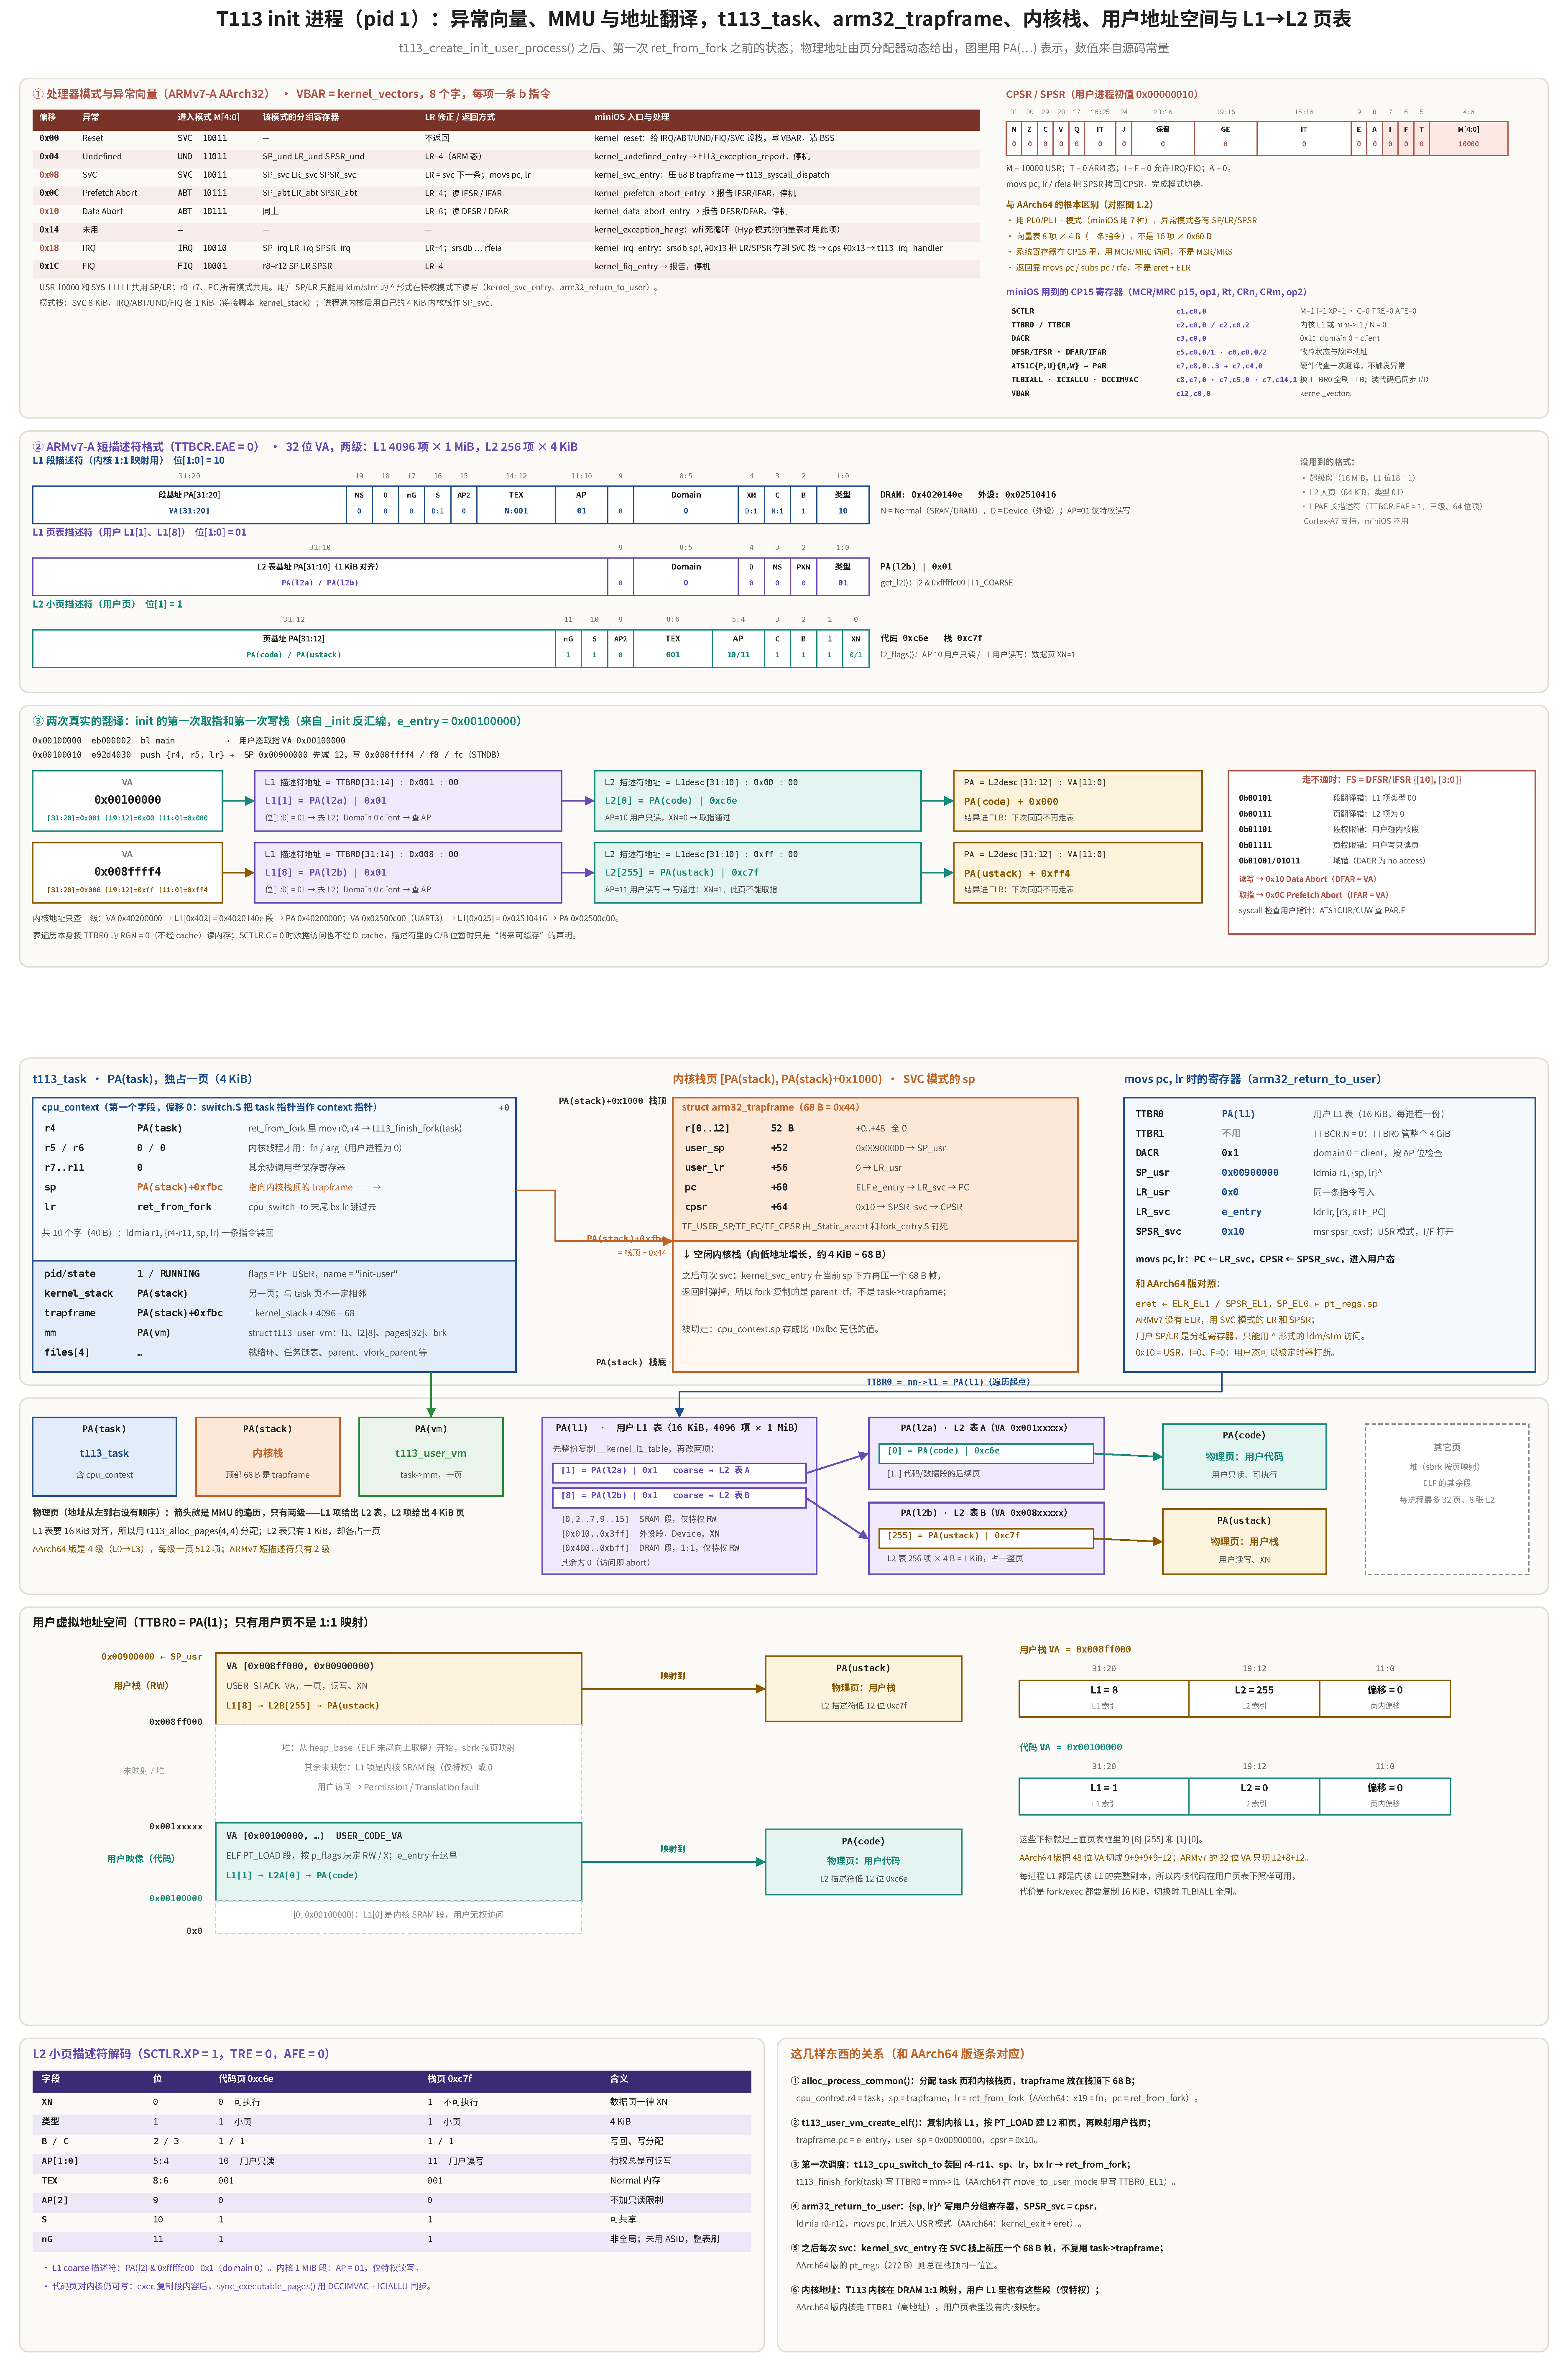
\includegraphics[width=\linewidth]{figures/t113-proc-vm-pid1.pdf}
  \caption{T113 init 进程：异常向量、MMU 与地址翻译，\code{t113\_task}、\code{arm32\_trapframe}、内核栈、用户地址空间与 L1→L2 页表}
  \label{fig:t113-proc-vm}
\end{figure}

\begin{figure}[p]
  \centering
  \includegraphics[width=\linewidth]{figures/bare-proc-vm-pid1_11.pdf}
  \caption{树莓派 AArch64 pid 1：\code{task\_struct}、\code{pt\_regs}、内核栈、用户地址空间与 L0→L3 页表}
  \label{fig:aarch64-proc-vm}
\end{figure}

两张图对照下来，差别集中在这几处：

\begin{table}[H]
\centering
\small
\begin{tabularx}{\linewidth}{>{\raggedright\arraybackslash}X>{\raggedright\arraybackslash}X>{\raggedright\arraybackslash}X}
\toprule
方面 & 树莓派 AArch64 & T113 ARMv7-A \\
\midrule
切换上下文 & x19–x29、fp、sp、pc（x19 = fn） & r4–r11、sp、lr（r4 = task，r5/r6 = 内核线程的 fn/arg） \\
用户寄存器帧 & \code{pt\_regs} 272 B，总在栈顶同一位置 & \code{arm32\_trapframe} 68 B，每次 svc 在当前 sp 下新压一个 \\
回到用户态 & \code{kernel\_exit} + \code{eret}，ELR\_EL1 / SPSR\_EL1 / SP\_EL0 & \code{ldmia \{sp, lr\}\textasciicircum{}} + \code{msr spsr} + \code{movs pc, lr} \\
页表 & 4 级（L0→L3），每级 512 项，48 位 VA & 2 级短描述符：L1 4096 项 × 1 MiB（16 KiB），L2 256 项 × 4 KiB \\
内核映射 & TTBR1\_EL1，高地址，用户页表里没有 & TTBCR.N = 0，每个用户 L1 都是内核 L1 的完整副本（段只允许特权访问） \\
用户布局 & 代码 0x400000，栈顶 0x8000000 & 代码 0x00100000，栈顶 0x00900000 \\
进入用户态时的状态寄存器 & SPSR = 0x3c0（EL0t，DAIF 全屏蔽） & CPSR = 0x10（USR，IRQ/FIQ 打开） \\
\bottomrule
\end{tabularx}
\end{table}

\subsubsection*{AArch32 的异常、MMU 与地址翻译}

\textbf{处理器模式和分组寄存器。} ARMv7-A 不用 AArch64 的 EL，而是用特权级 PL0/PL1（虚拟化扩展另有 PL2）加处理器模式。miniOS 用到其中 7 种：USR、SYS、SVC、IRQ、FIQ、ABT、UND；Cortex-A7 另有 MON（安全扩展）和 HYP（虚拟化扩展），miniOS 不用。模式号在 CPSR[4:0]。除 USR/SYS 共用一组外，每种异常模式都有自己的 SP、LR、SPSR（FIQ 还有自己的 r8–r12）。所以\code{kernel\_reset} 要依次 \code{cps} 进每种模式设栈（SVC 8 KiB，其余各 1 KiB）；用户态的 SP/LR 在特权模式下看不见，\code{kernel\_svc\_entry} 和 \code{arm32\_return\_to\_user}只能用 \code{stmia/ldmia \{sp, lr\}\textasciicircum{}} 这种带 \code{\textasciicircum{}} 的形式访问。

\textbf{异常向量。} \code{VBAR}（CP15 c12）指向 \code{kernel\_vectors}，表里是 8 条\code{b handler} 指令，每项 4 字节，按偏移 0x00 Reset、0x04 Undefined、0x08 SVC、0x0C Prefetch Abort、0x10 Data Abort、0x14 未用、0x18 IRQ、0x1C FIQ 排列。进入异常时硬件把返回地址放进该模式的 LR，旧 CPSR 放进 SPSR；LR 的偏移因异常而异（Undef/Prefetch/IRQ/FIQ 减 4，Data Abort 减 8，SVC 不用改）。返回也不是一条统一指令：SVC 用 \code{movs pc, lr}，IRQ 先用 \code{srsdb sp!, \#0x13} 把 LR\_irq 和SPSR\_irq 压到 SVC 栈，处理完再用 \code{rfeia sp!} 一次恢复 PC 和 CPSR。Undef、Abort、FIQ 在 miniOS 里只报告现场然后停机。

\textbf{CP15 与 MMU 配置。} 系统寄存器都在协处理器 CP15 里，用 \code{mcr/mrc p15, …}访问。\code{t113\_mmu\_init()} 写 TTBR0 = \code{\_\_kernel\_l1\_table}、TTBCR = 0（N = 0，TTBR0 覆盖整个 4 GiB，TTBR1 不参与）、DACR = 1（domain 0 为 client，按 AP位检查），再在 SCTLR 里打开 M、I、XP，清 TRE、AFE，并且暂不打开 C（D-cache）。内核 L1 全是 1 MiB 段，1:1 映射：0x000–0x00F MiB 是 SRAM（Normal），0x010–0x3FF MiB 是外设（Device、XN），0x400–0xBFF MiB 是 DRAM（Normal），都只允许特权访问（AP = 01）。

\textbf{短描述符和两级翻译。} 32 位 VA 拆成 [31:20] L1 索引、[19:12] L2 索引、[11:0] 页内偏移。

\begin{txtcode}
L1 描述符地址 = TTBR0[31:14] : VA[31:20] : 00
   位[1:0] = 10 → 段：PA = desc[31:20] : VA[19:0]            （内核，查一级就结束）
   位[1:0] = 01 → 页表：继续
L2 描述符地址 = L1desc[31:10] : VA[19:12] : 00
   位[1]   = 1  → 小页：PA = desc[31:12] : VA[11:0]
\end{txtcode}

每个用户 L1 都是内核 L1 的完整副本，只把 L1[1]（代码）和 L1[8]（栈）换成页表描述符。这一点与 Linux 在 ARM 短描述符下的做法相同：TTBCR.N = 0，每个进程的 pgd 都带一份内核映射。区别是 Linux 在同一页里还放了软件用的影子 PTE，miniOS 的 1 KiB L2 表则单独占一页。

\textbf{两次真实的翻译。} 从 \code{\_init} 的反汇编看，\code{e\_entry} = 0x00100000，第一条指令\code{bl main} 触发对 VA 0x00100000 的用户态取指：L1[1] → L2A[0] = PA(code) | 0xc6e，AP = 10（用户只读）、XN = 0，通过。\code{main} 的第一条指令 \code{push \{r4, r5, lr\}}在 SP = 0x00900000 时写 0x008ffff4–0x008fffff：L1[8] → L2B[255] = PA(ustack) | 0xc7f，AP = 11（用户读写），通过；同一页 XN = 1，不能取指。

\textbf{走不通时。} 翻译或权限检查失败，数据访问进 Data Abort（DFSR 给状态，DFAR给地址），取指进 Prefetch Abort（IFSR/IFAR）。FS 编码 0b00101/0b00111 是段/页翻译错，0b01101/0b01111 是段/页权限错。系统调用检查用户指针时，不让它真的出错，而是用 ATS1CUR/ATS1CUW（CP15 c7, c8）让硬件代查一次翻译，再看 PAR 的F 位（\code{t113\_mmu\_probe()}）。切换进程只换 TTBR0 并 TLBIALL 全刷，没有使用ASID（CONTEXTIDR）。



\subsection{子进程第一次运行：\code{ret\_from\_fork}}

\begin{txtcode}
t113_sched_tick() / t113_sched_yield()
+-- schedule_next()
    +-- 在就绪环里从 prev->ready_next 开始找 state == RUNNING
    |   +-- 一个都没有 → boot_context（kernel_boot 的 wfi 循环）
    +-- t113_current = next
    +-- switch_task_mm(next)            TTBR0 ← next->mm->l1 或内核 L1 表
    +-- t113_cpu_switch_to(prev, next)  switch.S
        +-- stmia r0, {r4-r11, sp, lr}  保存 prev
        +-- ldmia r1, {r4-r11, sp, lr}  装入 next：r4=task, sp=trapframe, lr=ret_from_fork
        +-- bx lr
            +-- ret_from_fork           fork_entry.S
                +-- t113_finish_fork(r4)
                |   +-- PF_KTHREAD → t113_switch_kernel_vm()
                |   +-- PF_USER    → t113_switch_user_vm(task->mm)
                +-- 内核线程：cpsie i; mov r0, r6; blx r5
                |   +-- fn(arg) 返回 → t113_task_exit()   state = IDLE, wfi
                +-- 用户进程：t113_task_trapframe(r4) → arm32_return_to_user(tf)
                    +-- ldmia {sp, lr}^        写 User 模式的 banked SP/LR
                    +-- lr  = tf->pc
                    +-- spsr = tf->cpsr        0x10 = User 模式，IRQ 打开
                    +-- ldmia r0-r12           r0 = 0
                    +-- movs pc, lr            CPSR ← SPSR，跳到 svc 的下一条
                        +-- 子进程在用户态从 fork()/vfork() 返回 0
\end{txtcode}

\code{r4/r5/r6} 是 miniOS 自己定的约定：它们是被调用者保存寄存器，\code{t113\_cpu\_switch\_to} 会原样恢复，所以可以用来把“任务指针、内核函数、参数”带到 \code{ret\_from\_fork}。AArch64 版本用的是 \code{x19/x20}，道理相同。

\subsection{vfork：父进程怎样等、怎样被唤醒}

\begin{txtcode}[basicstyle=\ttfamily\scriptsize]
 父进程 P                          调度器                      子进程 C
 vfork() - svc #0, r7 = 14 -→ t113_syscall_dispatch(tf)
   t113_vfork_user(tf)
     t113_kernel_clone(VM|VFORK)
       C.mm = P.mm（references = 2）
       C.vfork_parent = P
       P.state = WAITING
     t113_sched_yield() ------→ schedule_next()
                                P 不是 RUNNING，跳过
                                选中 C ----------------------→ ret_from_fork
                                                               用户态 vfork() 返回 0
                                                               exec("/bin/ls", argv)
                                                               +-- sys_exec()
                                                                   +-- 新建 vm，装入 ELF
                                                                   +-- C.mm = 新 vm
                                                                   +-- t113_vfork_complete(C)
                                                                   |   +-- P.state = RUNNING
                                                                   |   +-- C.vfork_parent = 0
                                                                   +-- 切 TTBR0 到新 vm
                                                                   +-- t113_user_vm_put(P 的 mm)
                                                                       references = 1
                                ...之后某次调度选中 P
 ←---------------------------- t113_sched_yield() 返回
 t113_vfork_user() 返回 C 的 pid
 用户态 vfork() 返回 C 的 pid
\end{txtcode}

\code{t113\_vfork\_complete()} 有两个调用点，对应 Linux 在 \code{mm\_release()} 里\code{complete(vfork\_done)} 的两种情况：

\begin{itemize}
  \item \code{sys\_exec()}（\code{src/kernel/syscall.c}）：子进程换上了自己的地址空间；
  \item \code{t113\_exit\_current()}（\code{sched/core.c}）：子进程没 exec 就退出了。
\end{itemize}

父进程用的是 \code{WAITING} 状态，不是忙等。\code{t113\_exit\_current()} 里，“父进程在WAITING 就改回 RUNNING”这条规则同时服务了 \code{wait()} 和 vfork。

\begin{note}
注意：vfork 的子进程在父进程的用户栈上运行。\code{user-t113/usys.S} 的 \code{\_\_sys\_vfork} 用 \code{push \{r7, lr\}} / \code{pop \{r7, pc\}}保存返回地址，\code{libc.c} 的 \code{vfork()} 又是 C 包装。子进程返回后再调用\code{exec()}，新的栈帧会落在同一片栈上，覆盖父进程还没弹出的返回地址。父进程恢复后从被改写的栈上返回，就会跳错地方。glibc 在 ARM 上用汇编写vfork，把返回地址留在寄存器里、不碰栈，原因就在这里。目前\code{user-t113/} 里还没有程序调用 \code{vfork()}；要用它，应先把包装改成不使用栈的汇编，或在子进程里直接内联 \code{svc}。
\end{note}

\subsection{地址空间：共享还是复制}

\begin{txtcode}[basicstyle=\ttfamily\scriptsize]
struct t113_user_vm（一页）
+-- references                      vfork 共享时为 2
+-- l1 --→ 16 KiB L1 表（4096 项，每项管 1 MiB）
|          +-- 内核区：创建时整表拷贝 __kernel_l1_table
|          +-- 用户区：指向 l2[]（最多 8 张 L2 粗页表）
+-- pages[32]  {va, pa, writable, executable}
|          代码 0x00100000 起，栈 0x008ff000–0x00900000，堆 [heap_base, brk)
+-- page_count / heap_base / brk

fork  : t113_user_vm_clone(src)
        +-- 新 vm 页 + 新 16 KiB L1（拷贝内核项）
        +-- 对 src->pages[i]：map_page(va, 同权限) + copy_bytes(4 KiB)
        +-- heap_base / brk 照抄
        +-- sync_executable_pages()       代码页逐行 DCCIMVAC，再 ICIALLU，保证取指看到新内容
vfork : child->mm = parent->mm; references++
exec  : 新建 vm，成功后 t113_user_vm_put(旧 vm)
wait  : 回收僵尸时 t113_user_vm_put(zombie->mm)
\end{txtcode}

T113 没有写时复制，fork 的代价正比于用户页数（最多 32 页，即 128 KiB 的memcpy）。这也是 vfork 存在的意义：shell 的“fork 后马上 exec”可以省掉这次拷贝。

\subsection{exit 与 wait}

\begin{txtcode}
t113_exit_current(status)                 T113_SYS_EXIT
+-- t113_vfork_complete(self)             没 exec 就退出的 vfork 子进程也要放行父进程
+-- 关闭 files[0..3]
+-- 子进程过继给 init_task                  与 xv6 reparent() 相同
|   +-- 有已是 ZOMBIE 的且 init 在 WAITING → 唤醒 init
+-- exit_status = status, state = ZOMBIE
+-- parent 在 WAITING → RUNNING
+-- t113_sched_yield()，不再返回

t113_wait_child(&status)                  T113_SYS_WAIT
+-- 循环
    +-- 扫 task_head 链表找 parent == current 的子进程
    +-- 有 ZOMBIE：摘链 → t113_user_vm_put(mm) → 释放 task/栈页 → 返回 pid
    +-- 一个子进程都没有 → -1
    +-- 否则 state = WAITING，yield，被 exit 唤醒后重扫
\end{txtcode}

\subsection{与 xv6 的进程创建对照}

xv6（这里对照的是 \code{xv6-aarch64/kernel/proc.c}）只有 \code{fork()}，没有 vfork 和clone，也没有内核线程。它的调用链：

\begin{txtcode}
sys_fork() → fork()                                  kernel/proc.c
+-- allocproc()
|   +-- 遍历 proc[NPROC] 找 UNUSED，持有 p->lock 返回
|   +-- pid = allocpid()
|   +-- trapframe = kstack + PGSIZE - sizeof(trapframe)   aarch64 移植放在内核栈顶
|   +-- pagetable = uvmcreate()
|   +-- context.x30 = forkret, context.sp = trapframe 处
+-- uvmcopy(p->pagetable, np->pagetable, p->sz)      逐页 kalloc + memmove，没有 COW
+-- np->sz = p->sz
+-- *(np->trapframe) = *(p->trapframe)
+-- np->trapframe->x0 = 0                            子进程返回 0
+-- ofile[i] = filedup(); cwd = idup()
+-- np->parent = p                                   持 wait_lock
+-- np->state = RUNNABLE

scheduler()                                          每个 CPU 一个调度循环
+-- swtch(&c->context, &p->context)
    +-- forkret()
        +-- release(&p->lock)                        scheduler 持锁切过来
        +-- 第一次：fsinit(ROOTDEV)                  文件系统初始化要能 sleep
        +-- usertrapret(tf) → eret 回 EL0
\end{txtcode}

\begin{table}[H]
\centering
\small
\begin{tabularx}{\linewidth}{l>{\raggedright\arraybackslash}X>{\raggedright\arraybackslash}X}
\toprule
方面 & xv6-aarch64 & T113 miniOS \\
\midrule
创建接口 & 只有 \code{fork()} & \code{t113\_kernel\_clone(flags)} 一个入口，派生 fork、vfork、内核线程 \\
进程表 & 静态 \code{proc[NPROC]}，每项一把 \code{p->lock} & 每个任务动态分配一页，\code{task\_head} 链表 + 就绪环，一把 \code{sched\_lock} \\
地址空间 & 4 级页表，\code{uvmcopy} 按 \code{p->sz} 逐页复制 & ARMv7 短描述符 L1/L2，\code{t113\_user\_vm\_clone} 按 \code{pages[]} 逐页复制 \\
共享地址空间 & 不支持 & \code{T113\_CLONE\_VM} + \code{references} 引用计数 \\
父进程等待 & 只有 \code{wait()}，用 sleep/wakeup 加通道 & \code{wait()} 和 vfork 都用 \code{WAITING} 状态，exit/exec 改回 \code{RUNNING} \\
第一次运行 & \code{forkret} → \code{usertrapret} & \code{ret\_from\_fork} → \code{t113\_finish\_fork} → \code{arm32\_return\_to\_user} \\
调度切换 & 进程 \ensuremath{\leftrightarrow} 每 CPU 的调度线程（两次 \code{swtch}） & 进程 \ensuremath{\leftrightarrow} 进程直接 \code{t113\_cpu\_switch\_to}，单核 \\
内核线程 & 无 & \code{T113\_CLONE\_KTHREAD}，\code{r5/r6} 带函数和参数 \\
返回值寄存器 & \code{trapframe->x0} & \code{trapframe->r[0]} \\
文件系统初始化 & 第一个进程的 \code{forkret} 里 \code{fsinit()} & \code{kernel\_boot()} 里在创建 init 之前挂好 \\
\bottomrule
\end{tabularx}
\end{table}

\subsection{与 Linux 的对照}

Linux 的 fork、vfork、clone、clone3 和 \code{kernel\_thread()} 最后都进\code{kernel\_clone(struct kernel\_clone\_args *)}：

\begin{txtcode}[basicstyle=\ttfamily\scriptsize]
fork()        → kernel_clone({ .exit_signal = SIGCHLD })
vfork()       → kernel_clone({ .flags = CLONE_VFORK | CLONE_VM, .exit_signal = SIGCHLD })
clone(flags...) → kernel_clone({ .flags = flags, .stack = newsp, ... })
kernel_thread → kernel_clone({ .flags = CLONE_VM | CLONE_UNTRACED, .fn = fn, .fn_arg = arg, .kthread = 1 })

kernel_clone()
+-- copy_process()          copy_mm / copy_files / copy_fs / copy_sighand / copy_thread
+-- CLONE_VFORK → p->vfork_done = &vfork（completion）
+-- wake_up_new_task(p)
+-- CLONE_VFORK → wait_for_vfork_done()   子进程 exec/exit 时 mm_release() → complete()
\end{txtcode}

T113 的做法是这条路径的缩小版：

\begin{itemize}
  \item \code{T113\_CLONE\_VM} 对应 \code{copy\_mm()} 里共享还是 \code{dup\_mm()}；
  \item \code{vfork\_parent} + \code{WAITING} 对应 \code{vfork\_done} completion；
  \item \code{t113\_vfork\_complete()} 对应 \code{mm\_release()} 里的 \code{complete\_vfork\_done()}；
  \item 文件描述符总是逐个加引用，相当于 Linux 不带 \code{CLONE\_FILES} 时的\code{dup\_fd()}；
  \item 没有线程，因为没有用户态 clone 系统调用，也不能给子进程另指用户栈。
\end{itemize}

\subsection{树莓派 AArch64 与 T113 ARMv7 的实现区别}

\begin{table}[H]
\centering
\small
\begin{tabularx}{\linewidth}{>{\raggedright\arraybackslash}X>{\raggedright\arraybackslash}X>{\raggedright\arraybackslash}X}
\toprule
方面 & 树莓派（前文） & T113 \\
\midrule
创建函数 & \code{copy\_process(clone\_flags, fn, arg, stack)}，\code{clone\_flags} 复用 \code{PF\_KTHREAD} & \code{t113\_kernel\_clone(flags, parent\_tf, name, fn, arg)}，策略标志与 \code{PF\_*} 分开 \\
首次运行寄存器 & \code{x19 = fn}、\code{x20 = arg}，\code{pc = ret\_from\_fork} & \code{r4 = task}、\code{r5 = fn}、\code{r6 = arg}，\code{lr = ret\_from\_fork} \\
用户上下文 & \code{pt\_regs}（x0–x30、sp、pc、pstate） & \code{arm32\_trapframe}（r0–r12、user\_sp、user\_lr、pc、cpsr，68 B） \\
进入内核 & \code{svc \#0}，异常级 EL0 → EL1，\code{x8} 是调用号 & \code{svc \#0}，User → SVC 模式，\code{r7} 是调用号 \\
回用户态 & \code{kernel\_exit} → \code{eret}（ELR/SPSR\_EL1） & \code{ldmia \{sp,lr\}\textasciicircum{}} + \code{movs pc, lr}（SPSR\_svc） \\
用户页表 & \code{TTBR0\_EL1}，4 KiB 粒度多级表 & \code{TTBR0}，16 KiB L1 + 1 KiB L2，内核项拷进每张 L1 \\
用户进程来源 & 内核把嵌入的镜像拷进去（\code{move\_to\_user\_mode}） & 从根文件系统读 ELF（\file{/init}、\code{exec}） \\
fork/vfork 系统调用 & 无 & 有，另有 wait/exit/exec/sbrk \\
\bottomrule
\end{tabularx}
\end{table}
